\documentclass{article}
\usepackage{amsmath}
\usepackage{amssymb}
\usepackage{graphicx}
\usepackage{hyperref}
\usepackage[version=4]{mhchem}

\title{Problem 9}
\date{}

\begin{document}
\maketitle

\section*{Problem}
(1996 Mathcounts National Sprint Problem 25) In the diagram, circle \(Q\) is congruent to circle W , and both are tangent to circle \(O\) and to each other. Circle \(S\) and circle \(T\) are congruent and\\
\centering
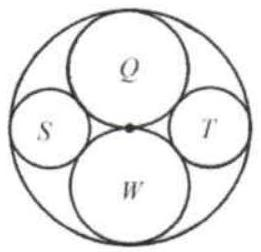
\includegraphics[width=\textwidth]{images/problem_image_1.jpg}\\
are tangent to circle \(O\), to circle \(Q\) and to circle \(W\). Find the ratio of the area of the smallest circle to the largest circle.

\section*{Solution}
1: 9.
Let the radius of the circle \(O\) be \(R\), the radius of the circle \(Q\) be \(r_{1}\), and the radius of the circle \(S\) be \(r_{2}\). We know that \(r_{1}=\frac{R}{2}\).\\
By the Pythagorean Theorem,\\
\(\left(R-r_{2}\right)^{2}=r_{1}^{2}+\left(r_{1}+r_{2}\right)^{2} \Rightarrow R^{2}-2 R r_{2}=2 r_{1} r_{2} \Rightarrow\)\\
\centering
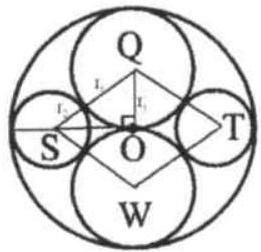
\includegraphics[width=\textwidth]{images/reasoning_image_1.jpg}\\
\(R^{2}-2 R r_{2}=2 r_{1} r_{2} \Rightarrow r_{2}=\frac{R}{3}\)\\
The ratio of the areas of the smallest circle and largest circle is\\
\(\frac{\pi r_{2}{ }^{2}}{\pi R^{2}}=\frac{r_{2}{ }^{2}}{R^{2}}=\frac{\left(\frac{R}{3}\right)^{2}}{R^{2}}=\frac{1}{9}\).\\

\end{document}
